\
A \textbf{function generator} is an electronic device used to generate various types of electrical waveforms over a wide range of frequencies. It is commonly used in electronics testing, development, and troubleshooting.

\begin{figure}[h!]
    \centering
    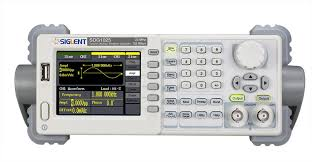
\includegraphics[width=0.6\textwidth]{figures/functiongenerator.jpeg}
    \caption{Function Generator}
    \label{fig:sample_image}
\end{figure}
\subsection{Key Features of a Function Generator}
\begin{itemize}
    \item \textbf{Waveform Types:}
    \begin{itemize}
        \item \textit{Sine wave:} Smooth periodic oscillations.
        \item \textit{Square wave:} Alternates between high and low levels, used in digital circuits.
        \item \textit{Triangle wave:} Linear rise and fall, used in modulation and testing.
        \item \textit{Sawtooth wave:} Sharp rise and slow fall or vice versa.
        \item \textit{Pulse wave:} Short-duration signal for timing and control purposes.\\
    \end{itemize}
    \item \textbf{Frequency Range:} Typically operates over a range from a few Hz to several MHz.
    \item \textbf{Amplitude Control:} Users can adjust the output signal's amplitude.
    \item \textbf{DC Offset:} Allows adding a constant voltage to the waveform.
    \item \textbf{Modulation:} Some function generators can apply modulation techniques like AM (Amplitude Modulation) or FM (Frequency Modulation).
    \item \textbf{Output Impedance:} Generally 50 ohms, matching typical test equipment.
\end{itemize}
\subsection{Applications}
\begin{itemize}
    \item \textbf{Testing Circuits:} Used to test amplifiers, filters, and other electronic circuits.
    \item \textbf{Signal Injection:} Provides input signals for troubleshooting and diagnostics.
    \item \textbf{Waveform Generation:} Generates waveforms for experimentation in labs.
    \item \textbf{Modulation and Timing:} Helps simulate signals for communication systems.
\end{itemize}

In advanced setups, function generators are often replaced by \textbf{arbitrary waveform generators (AWGs)} for more complex signal requirements.
